\documentclass{book}
\usepackage[a4paper,
            left=0.5in,
            right=0.5in,
            top=0.5in,
            bottom=0.5in,
            ]{geometry}
\usepackage{minted}
\setlength{\parindent}{0pt}
\usepackage{graphicx}
\graphicspath{{.}}

\begin{document}
{\Huge \textbf{Lab 5: Swing and JavaFX}}
\\
\par
{
    \large
    \textbf{Objectives:}
    \begin{itemize}
        \item Use Different layouts in Swing and JavaFX
        \item Learn GUI controls in Swing and JavaFX
        \item Learn about event handling and listener Interfaces
    \end{itemize}

    \textbf{Programs:}
    \begin{enumerate}
        \item \textbf{Program 1 School Management System}
        \begin{itemize}
            \item react/Reactive.java
            \inputminted{java}{react/Reactive.java}
            \item react/Clearable.java
            \inputminted{java}{react/Clearable.java}
            \item react/Renderable.java
            \inputminted{java}{react/Renderable.java}
            \item RegistrationForm.java
            \inputminted{java}{RegistrationForm.java}
        
            \par

            \textbf{Output:}
            \begin{itemize} 
                \item { \textbf{Main Frame}
                    \center{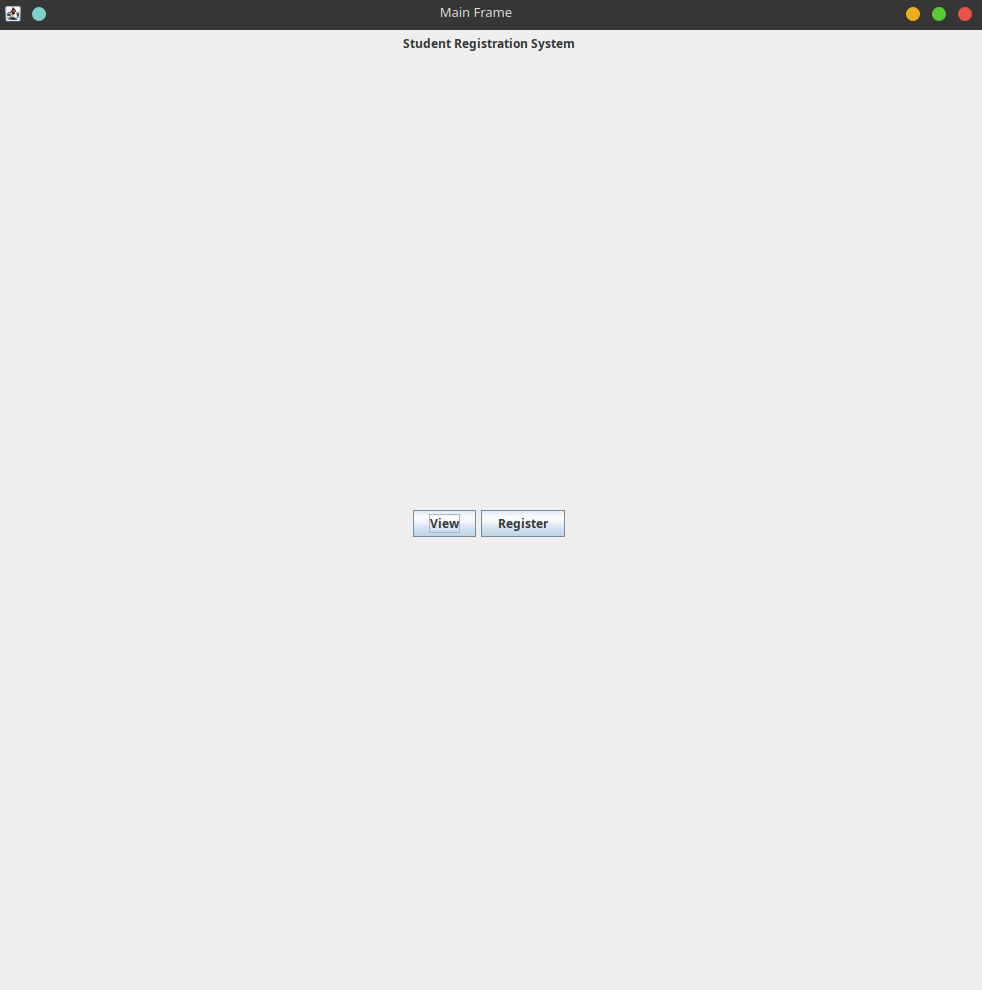
\includegraphics[width=0.5\textwidth]{MainFrame.png}}
                }
                \item{ \textbf{Registration Frame}
                    \center{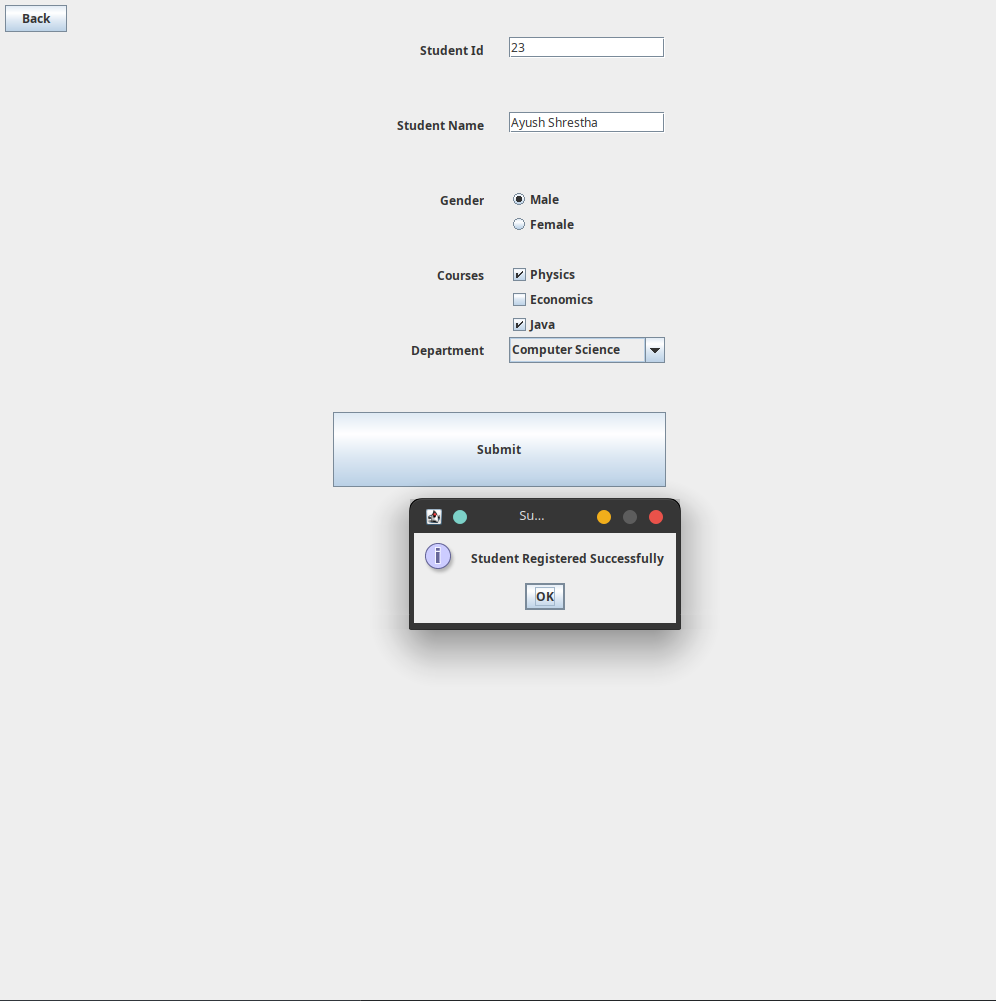
\includegraphics[width=0.5\textwidth]{RegistrationFrame.png}}
                }
                \item{ \textbf{Registration Error}
                    \center{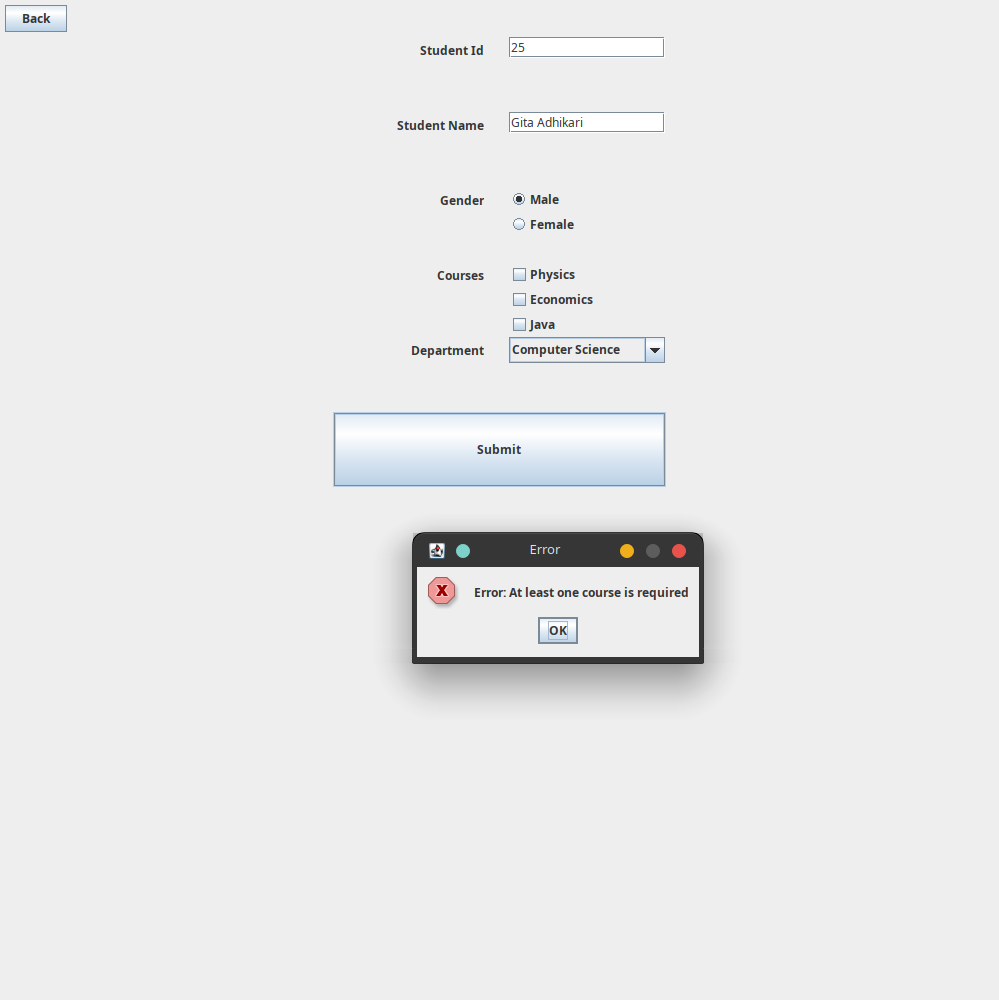
\includegraphics[width=0.5\textwidth]{RegistrationError.png}}
                }
                \item{ \textbf{View Frame}
                    \center{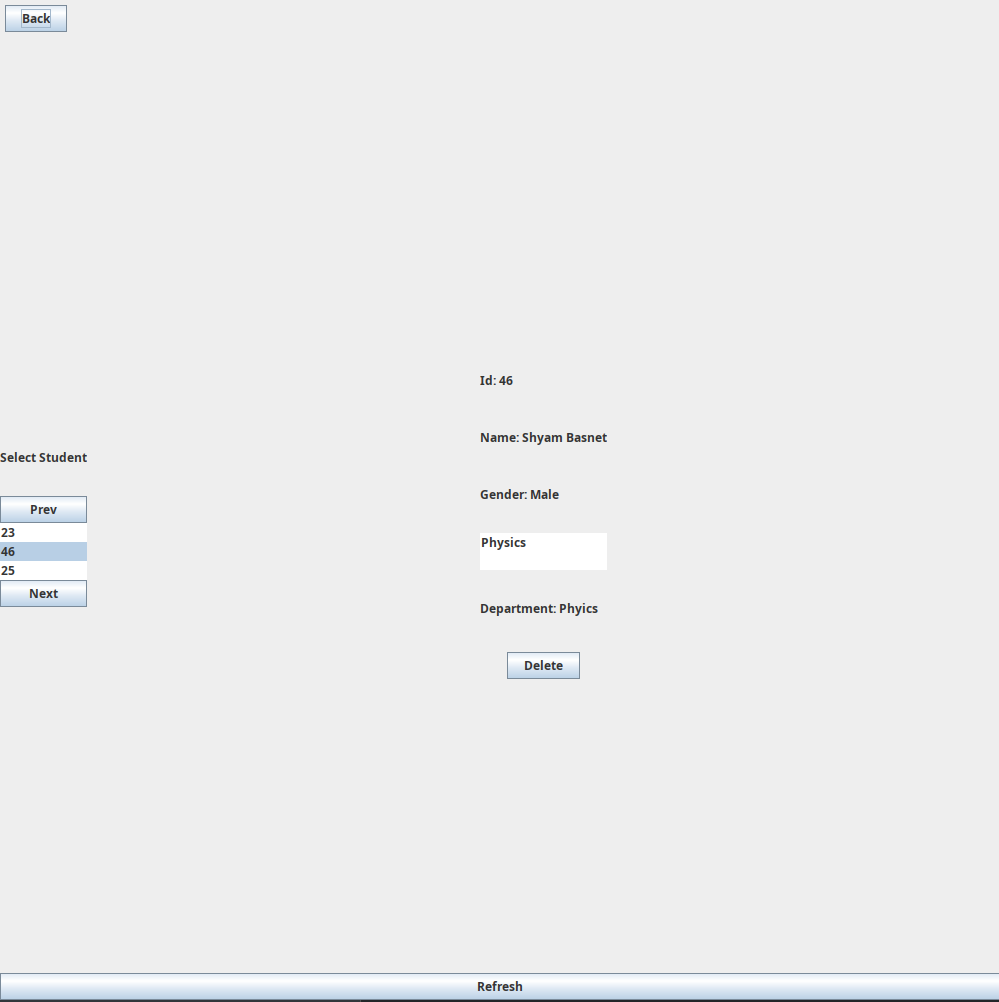
\includegraphics[width=0.5\textwidth]{ViewFrame.png}}
                }
            \end{itemize}


        \end{itemize}

        \item \textbf{Program 2: JavaFX program}

        \begin{minted}{java}
    package org.mdhe.jfx;
    import javafx.application.Application;
    import javafx.geometry.Insets;
    import javafx.geometry.Pos;
    import javafx.scene.Node;
    import javafx.scene.Parent;
    import javafx.scene.Scene;
    import javafx.scene.control.Button;
    import javafx.scene.control.Tab;
    import javafx.scene.control.TabPane;
    import javafx.scene.control.TextField;
    import javafx.scene.image.Image;
    import javafx.scene.image.ImageView;
    import javafx.scene.layout.*;
    import javafx.scene.paint.Color;
    import javafx.scene.text.Text;
    import javafx.stage.Stage;



    public class HelloApplication extends Application {
        @Override
        public void start(Stage stage){
            stage.setTitle("WOW");

            Scene newScene = new Scene(createContent(), 300, 300);

            stage.setScene(newScene);

            stage.show();
        }

        private Parent createContent() {
            Tab BMItab = new Tab("BMI", createBMITab());

            BMItab.setClosable(false);
            Tab InterestTab = new Tab("Interest", createInterestTab());
            InterestTab.setClosable(false);
            Tab ImageTab = new Tab("Image",createImageTab());
            ImageTab.setClosable(false);

            TabPane tabPane = new TabPane(BMItab, InterestTab, ImageTab);

            return tabPane;

        }

        private Node createBMITab() {


            TextField height = new TextField();
            height.setPromptText("Height in meters");
            TextField weight = new TextField();
            weight.setPromptText("Weight in KG");
            Button calculate = new Button("Calculate");

            Text Result = new Text();
            Result.setFill(Color.valueOf("green"));
            calculate.setOnAction(e -> {
                double h = Double.parseDouble(height.getText());
                double w = Double.parseDouble(weight.getText());
                double bmi = w / (h * h);
                Result.setText(String.valueOf(bmi));
            });

            VBox v = new VBox(
                    height,
                    weight,
                    calculate,
                    Result
            );
            v.setAlignment(Pos.TOP_CENTER);
            v.setSpacing(5);


            VBox details = new VBox(
                    new Text("BMI VALUES"),
                    new Text("Underweight less than 18.5"),
                    new Text("Normal between 18.5 and 24.9"),
                    new Text("Overweight between 25 and 29.9"),
                    new Text("Obese 30 or greater")
            );
            details.setSpacing(5);

            HBox h = new HBox(v,
                    details
            );
            h.setSpacing(20);
            h.setPadding(new Insets(10, 20, 0, 20));

            return h;
        }

        private Node createInterestTab() {


            GridPane gridPane = new GridPane(10, 5);

            gridPane.setPadding(new Insets(10, 20, 0, 20));

            TextField principal = new TextField();
            principal.setPromptText("Enter principal");

            TextField time = new TextField();
            time.setPromptText("Enter Time");


            TextField rate = new TextField();
            rate.setPromptText("Rate");

            TextField result = new TextField();
            result.setEditable(false);
            result.setFocusTraversable(false);

            Button calculate = new Button("Calculate");
            calculate.setOnAction(e -> {
                double p = Double.parseDouble(principal.getText());
                double t = Double.parseDouble(time.getText());
                double r = Double.parseDouble(rate.getText());
                result.setText(String.valueOf((p * t * r) / 100));
            });


            gridPane.add(principal, 0, 0);
            gridPane.add(rate, 0, 1);
            gridPane.add(time,0,2);
            gridPane.add(calculate, 0, 3);
            gridPane.add(result, 1, 0, 1, 4);


            return gridPane;
        }

        private Node createImageTab(){
        GridPane grid = new GridPane(10,10);
        grid.setPadding(new Insets(10,20,0,20));


        Image img = new Image("file:eiffel.jpg",0,0,true,true);
        ImageView imgView = new ImageView(img);
        imgView.setPreserveRatio(true);
        imgView.setFitWidth(200);
        grid.add(imgView,0,0);

        Text hojlundInfo = new Text("Picture of eiffel Tower");
        grid.add(hojlundInfo,1,0);


        Image java = new Image("https://images.ctfassets.net/1aemqu6a6t65/" +
        "79p5qaxQZWOIChawwXAkea/106da073c4ccf4e4d92966a1b2aff4e0/statue-of-" +
        "liberty-photo-julienne-schaer-nyc-and-" +
        "company-003-3?w=1200&h=800&q=75",0,0,true,true);

        ImageView javaImgView = new ImageView(java);
        javaImgView.setPreserveRatio(true);
        javaImgView.setFitWidth(200);
        grid.add(javaImgView,1,1);

        Text javaInfo = new Text("Statue Of Liberty");
        grid.add(javaInfo,0,1);


        return grid;
    }

        public static void main(String[] args) {
            launch();
        }
    }
        
    \end{minted}
    \par
    \textbf{Output:}
    \begin{itemize} 
        \item { \textbf{BMI Tab}
            \center{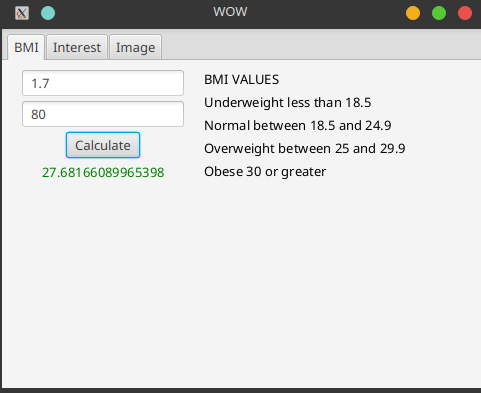
\includegraphics[width=0.5\textwidth]{bmiTab.png}}
        }
        \item{ \textbf{Interest Tab}
            \center{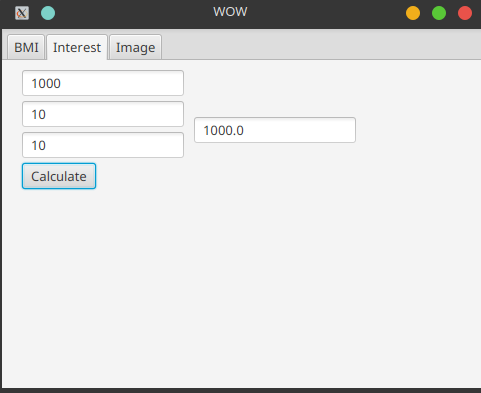
\includegraphics[width=0.5\textwidth]{InterestTab.png}}
        }
        \item{ \textbf{Image Tab}
            \center{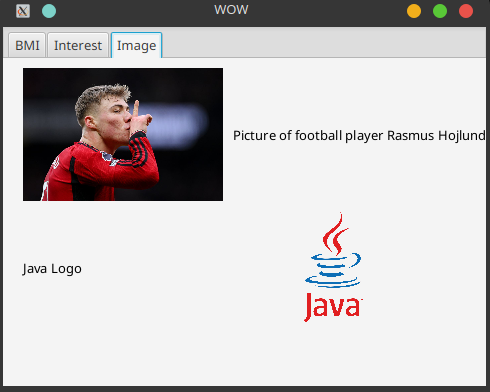
\includegraphics[width=0.5\textwidth]{imageTab.png}}
        }
    \end{itemize}
    \end{enumerate}
    \par
    \textbf{Conclusion:}
    \begin{itemize}
        \item We learned about different layouts in Swing and JavaFX
        \item We learned about GUI controls in Swing and JavaFX
        \item We learned about event handling and listener Interfaces
    \end{itemize}
}

\end{document}
